\documentclass{scrartcl}
\usepackage{tikz}
\usetikzlibrary{decorations.markings}
\tikzset{->-/.style={decoration={markings,mark=at position #1 with {\arrow{>}}},postaction={decorate}}}

\begin{document}

%\begin{figure}
%	\centering
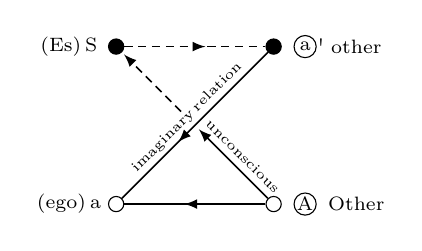
\begin{tikzpicture}[>=latex]
\node[circle,draw=black, fill=black, inner sep=0pt,minimum size=5.5pt] (S) at (0,2) {};
\node[circle,draw=black, fill=black, inner sep=0pt,minimum size=5.5pt] (a) at (2,2) {};
\node[circle,draw=black, fill=white, inner sep=0pt,minimum size=5.5pt] (E) at (0,0) {};
\node[circle,draw=black, fill=white, inner sep=0pt,minimum size=5.5pt] (A) at (2,0) {};

%outer lines
\draw [->-=.575, semithick, densely dashed] (S)--(a);	 		 %S--a
\draw [->-=.615, semithick] 				(a)--(E);		 	 %a--E
\draw [->-=.575, semithick] 			    (A)--(E);			 %Z--S
\draw [->, semithick]  						(A)--(1.05,0.95);	 %A--i
\draw [->, semithick, densely dashed] (0.825,1.175)--(0.1,1.9);  %i--S

%circles
\node (C) at (2.4,0) {{\scriptsize A}};	\draw (C) circle (4pt);
\node (c) at (2.4,2) {{\scriptsize a}};	\draw (c) circle (4pt);
\node     at (2.63,2) {{\scriptsize \rotatebox{22}{$^\prime$}}};

%labels
\node at (-0.6,0) {{\scriptsize (ego)$\,$a}};
\node at (3.05,0) {{\scriptsize Other}};
\node at (-0.6,2) {{\scriptsize (Es)$\,$S}};
\node at (3.05,2) {{\scriptsize other}};
%
\node at (1.61,0.61) {\rotatebox{-45}{{\tiny unconscious}}};
\node at (0.9,1.1)   {\rotatebox{45}{{\tiny imaginary$\,$relation}}};
\end{tikzpicture}
%	\caption{Lacan's Schema L}
%\end{figure}

\vspace{0.75cm}

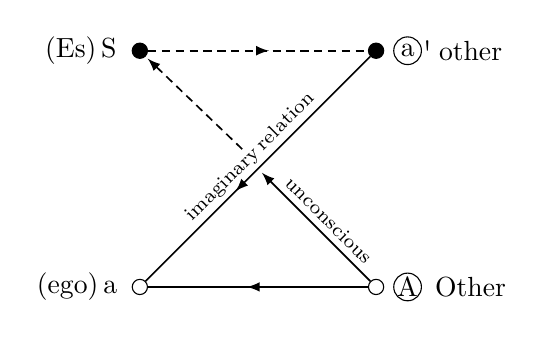
\begin{tikzpicture}[>=latex]
\node[circle,draw=black, fill=black, inner sep=0pt,minimum size=5.5pt] (S) at (0,3) {};
\node[circle,draw=black, fill=black, inner sep=0pt,minimum size=5.5pt] (a) at (3,3) {};
\node[circle,draw=black, fill=white, inner sep=0pt,minimum size=5.5pt] (E) at (0,0) {};
\node[circle,draw=black, fill=white, inner sep=0pt,minimum size=5.5pt] (A) at (3,0) {};

%outer lines
\draw [->-=.55, semithick, densely dashed] (S)--(a);	 		 %S--a
\draw [->-=.6, semithick] 				   (a)--(E);		 	 %a--E
\draw [->-=.55, semithick] 				   (A)--(E);			 %Z--S
\draw [->, semithick]  					   (A)--(1.55,1.45);	 %A--i
\draw [->, semithick, densely dashed] (1.3,1.75)--(0.1,2.9); 	 %i--S

%circles
\node (C) at (3.4,0) {A};	\draw (C) circle (5pt);
\node (c) at (3.4,3) {a};	\draw (c) circle (5pt);
\node     at (3.685,3) {\rotatebox{22}{$^\prime$}};

%labels
\node at (-0.8,0)  {(ego)$\,$a};
\node at (4.2,0)   {Other};
\node at (-0.75,3) {(Es)$\,$S};
\node at (4.2,3)   {other};
%
\node at (2.4,0.85) {\rotatebox{-45}{{\scriptsize unconscious}}};
\node at (1.4,1.65) {\rotatebox{45}{{\scriptsize imaginary$\,$relation}}};
\end{tikzpicture}

\end{document}
